\subsection{\texorpdfstring{Functions of class \(C^{r,s}\)}{Functions of class C\^{}\{r,s\}}}

In this no., E denotes a real Banach space, F₁ and F₂ Banach spaces over K, V an open subset of E × F₁ and f a map from V to F₂. One endows E, F₁ and F₂ with norms compatible with their Banach space structures.

15.1.1 (“Differentiable case”). One assumes K = R and \(s \neq \omega\) . We say that f is of class \(C_{R}^{r,s}\) (or simply \(C^{r,s}\) ) if it possesses iterated partial derivatives \(D_{E}^{p}D_{F_{1}}^{q}f\) (1.7.2) continuous for every pair of positive integers \((p,q)\) such that \(p \leqslant r\) and \(p + q \leqslant s\) . It is equivalent to say that the iterated partial derivatives \(D_{F_{1}}^{q}f\) exist and are of class \(C^{r}\) for every integer q such that \(0 \leqslant q \leqslant s - r\) . If s = r, this is equivalent to saying that f is of class \(C^{r}\) ; if \(s \geqslant r + 1\) , this is equivalent to saying that f is of class \(C^{r}\) and \(D_{F_{1}}f\) of class \(C^{r,s-1}\) .

If f is of class \(C^{r,s}\) and if \(p \leqslant r, p + q + 1 \leqslant s\) , the function \(D_{E}^{p}D_{F_{1}}^{q}f\) has a partial derivative with respect to \(F_{1}\) given by:

\[
\mathbf {D} _ {\mathbf {F} _ {1}} (\mathbf {D} _ {\mathbf {E}} ^ {p} \mathbf {D} _ {\mathbf {F} _ {1}} ^ {q} f) = \mathbf {D} _ {\mathbf {E}} ^ {p} \mathbf {D} _ {\mathbf {F} _ {1}} ^ {q + 1} f.\tag{1}
\]

15.1.2 (“Analytic case”). We assume \(s = \omega\) . For every integer \(k \geqslant 0\) , denote by \(\mathbf{P}_{k}(\mathbf{F}_{1}; \mathbf{F}_{2})\) the space of continuous homogeneous polynomials of degree \(k\) on \(\mathbf{F}_{1}\) with values in \(\mathbf{F}_{2}\) , equipped with the norm defined in the Appendix of the first fascicle, p. 88, A.2.

One says that \(f\) is of class \(\mathbf{C}_{\mathbf{K}}^{r,\omega}\) (or simply \(\mathbf{C}^{r,\omega}\) if there is no ambiguity about K) if, for every point \((x_{0},y_{0})\in\mathbf{V}\), there exist a neighborhood U of \(x_{0}\) in E, real numbers \textgreater and \(\geqslant\), and functions \(h_{k}\colon\mathbf{U}\to\mathbf{P}_{k}(\mathbf{F}_{1};\mathbf{F}_{2})\) (\(k\in\mathbf{N}\)), of class \(\mathbf{C}^{r}\) (for the differentiable-manifold structure underlying the structure of the K-manifold \(\mathrm{P}_{k}(\mathrm{F}_{1};\mathrm{F}_{2})\)), such that:

\begin{enumerate}
\def\labelenumi{(\roman{enumi})}
\item
  \(\mathbf{U} \times (y_0 + \mathbf{B}(\mathbf{R})) \subset \mathbf{V}\) , where \(\mathbf{B}(\mathbf{R})\) is the open ball of radius \(\mathbf{R}\) in \(\mathbf{F}_1\) ;
\item
  if \(x \in \mathbf{U}\) and \(p \leqslant r\) , one has \(\sum_{k=0}^{\infty} \| D^p h_k(x) \| R^k \leqslant M\) ;
\item
  if \(\mathrm{si} x \in \mathrm{U}\) and \(t \in \mathrm{B}(\mathbb{R})\) , one has \(\sum_{k=0}^{\infty} h_k(x)(t) = f(x, y_0 + t)\) .
\end{enumerate}

These properties imply:

\begin{enumerate}
\def\labelenumi{(\roman{enumi})}
\setcounter{enumi}{3}
\tightlist
\item
  For every \(t \in \mathbf{B}(\mathbf{R})\) , the function \(x \mapsto f(x, y_0 + t)\) is of class \(\mathbf{C}^{r}\) in U, and one has
\end{enumerate}

\[
\mathbf {D} _ {\mathbb {E}} ^ {p} f (x, y _ {0} + t) = \sum_ {k = 0} ^ {\infty} \mathbf {D} ^ {p} h _ {k} (x) (t) \quad \text { if } p \leqslant r \text { and } x \in \mathrm{U}.\tag{2}
\]

One does not change the definition of functions of class \(C^{r,\omega}\) if one replaces condition (ii) above by one of the following two conditions:

(ii') The \(h_k\) define a morphism of class \(C^r\) from U into the real Banach space underlying the K-Banach space \(\mathcal{H}_{\mathbb{R}}(\mathrm{F}_1; \mathrm{F}_2)\) (3.1.1 and 3.1.2).

(ii'') The \(h_k\) define a morphism of class \(C'\) from U into the real Banach space underlying the K-Banach space \(\tilde{\mathcal{H}}_R(F_1; F_2)\) (3.1.5).

15.1.3. Suppose K = R. For f to be of class \(C_{R}^{r,\omega}\) , it is necessary and sufficient that f be of class \(C^{r,\infty}\) (15.1.1) and that, for every \((x_{0}, y_{0}) \in V\) , there exists a neighborhood \(V_{0}\) of \((x_{0}, y_{0})\) in V and positive real numbers A and M such that

\[
\frac {1}{q !} \left\| \mathrm{D} _ {\mathbf {E}} ^ {p} \mathrm{D} _ {\mathbf {F} _ {1}} ^ {q} f (x, y) \right\| \leqslant \mathrm{A}. \mathrm{M} ^ {q}\tag{3}
\]

for all \(p \leqslant r\) , every \(q \geqslant 0\) and every \((x, y) \in V_0\) .

15.1.4. Suppose K = C. For f to be of class \(C_{C}^{r,\omega}\) , it is necessary and sufficient that the following two conditions be satisfied:

\begin{enumerate}
\def\labelenumi{\alph{enumi})}
\item
  f is of class \(C_{R}^{r,\omega}\) for the real structures underlying \(F_{1}\) and \(F_{2}\) .
\item
  For every \((x, y) \in \mathbf{V}\) , \(\mathbf{D}_{\mathbb{F}_1} f(x, y)\) is a \(\mathbf{C}\)-linear map from \(\mathbf{F}_1\) to \(\mathbf{F}_2\) .
\end{enumerate}

When \(F_{1}\) is of finite dimension, one may replace a) by:

\(\mathit{a}^{\prime})\) \(f\) is of class \(C^{r}\) .

15.1.5. The set of maps of class \(\mathbf{C}^{r,s}\) from V into \(\mathbf{F}_2\) does not depend on the choice of norms on E, \(\mathbf{F}_1\) , \(\mathbf{F}_2\) .

15.1.6. Let B be a differentiable manifold of class \(C^{r}\) , let W be an open subset of \(B \times F_{1}\) , and let \(\rho\) be a map from W into \(F_{2}\) . Let \(c = (\mathrm{U}, \varphi, \mathrm{E}_{c})\) be a chart of the manifold B. Denote by \(W_{c}\) the open subset of \(E_{c} \times F_{1}\) that is the image under \(\varphi \times Id_{F_{1}}\) of \(W \cap (\mathrm{U} \times F_{1})\) and let \(\rho_{c}\) be the map from \(W_{c}\) to \(F_{2}\) such that

\[
\rho_{c}(\varphi(x),y) = \rho(x,y) \quad \text { if } \quad (x,y) \in \mathbf{W} \cap (\mathbf{U} \times \mathbf{F}_{1}).
\]

The map \(\rho\colon\mathbf{W}\to\mathbf{F}_{2}\) is said to be of class \(\mathbf{C}^{r,s}\) if, for every chart \(c\) of the manifold B, the map \(\rho_{c}\colon\mathbf{W}_{c}\to\mathbf{F}_{2}\) is of class \(\mathbf{C}^{r,s}\) in the sense of 15.1.1 and 15.1.2; it suffices that this condition be satisfied for a family of charts whose domains cover B. Such a map \(\rho\) is of class \(\mathbf{C}^{r}\) (for the real structures underlying \(\mathbf{B}\times\mathbf{F}_{1}\) and \(\mathbf{F}_{2}\)); its restriction to the set \(\mathbf{W}\cap(\{b\}\times\mathbf{F}_{1})\) is a K-morphism of class \(\mathbf{C}^{s}\) for every \(b\in\mathbf{B}\) .

15.1.7. Let \(\mathbf{B}_1\) and \(\mathbf{B}_2\) be differentiable manifolds of class \(\mathbf{C}^r\) , and let \(g: \mathbf{B}_1 \to \mathbf{B}_2\) be a

\pandocbounded{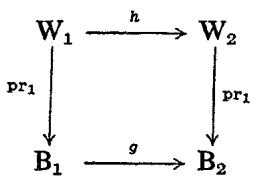
\includegraphics[keepaspectratio]{images/part001_9c3df15b.jpg}}

morphism of class \(\mathbf{C}^{r}\) . Let \(\mathbf{W}_{1}\) (resp. \(\mathbf{W}_{2}\)) be an open subset of \(\mathbf{B}_{1}\times\mathbf{F}_{1}\) (resp. of \(\mathbf{B}_{2}\times\mathbf{F}_{2}\)) and let \(h:\mathbf{W}_{1}\to\mathbf{W}_{2}\) be a map. We say that \(h\) is a \(g\)-morphism of class \(\mathbf{C}^{r,s}\) if \(\mathrm{pr}_{1}\circ h=g\circ\mathrm{pr}_{1}\) and if \(\mathrm{pr}_{2}\circ h\) is a map of class \(\mathbf{C}^{r,s}\) (15.1.6) from \(\mathbf{W}_{1}\) to \(\mathbf{F}_{2}\) .

Similarly, let \(B_{3}\) be a manifold of class \(C^{r}\) , let \(W_{3}\) be an open subset of \(B_{3} \times F_{3}\) , where \(F_{3}\) is a Banach K-space, and let \(g'\) be a morphism of class \(C^{r}\) from \(B_{2}\) to \(B_{3}\) . If h (resp.

\(h^{\prime})\) is a \(g\) -morphism (resp. \(g^{\prime}\) -morphism) of class \(\mathbf{C}^{r,s}\) of \(\mathbf{W}_1\) to \(\mathbf{W}_2\) (resp. of \(\mathbf{W}_2\) to \(\mathbf{W}_3\) ), the composite \(h^{\prime} \circ h\) is a \((g^{\prime} \circ g)\) -morphism of class \(\mathbf{C}^{r,s}\) of \(\mathbf{W}_1\) to \(\mathbf{W}_3\) .

